\label{key}\documentclass[letterpaper, 12pt,oneside]{article}
\usepackage{amsmath}
\usepackage{graphicx}
\usepackage{xcolor}
\graphicspath{{Imagenes/}}
\usepackage[utf8]{inputenc}
\usepackage{listings}
\usepackage[hidelinks]{hyperref}

\title{\Huge Taller de Herramientas Computacionales}
\author{Josué Artemio Hernández Rodríguez}
\date{24/Enero/2019}

\begin{document}
	\maketitle
	\begin{center}
		
\includegraphics[scale=0.7]{3.jpg}
	\end{center}

	\newpage
	
	\title{\huge \textit{Bitácora problema 7 }}\\

	Este problema es similar al anterior,salvo que ademas te pide calcular cual es el numero mayor y menor de todos. Me costo mucho trabajo, y el código me quedo bastante largo ya use bastantes condiciones comparando todos los números, es decir con \textit{if y else} anidados uno con otro, pude usar \textit{elif} pero no se hubiera acortado tanto. Al final funciona que era lo que se pedía.
	 

	\begin{figure}[h]
		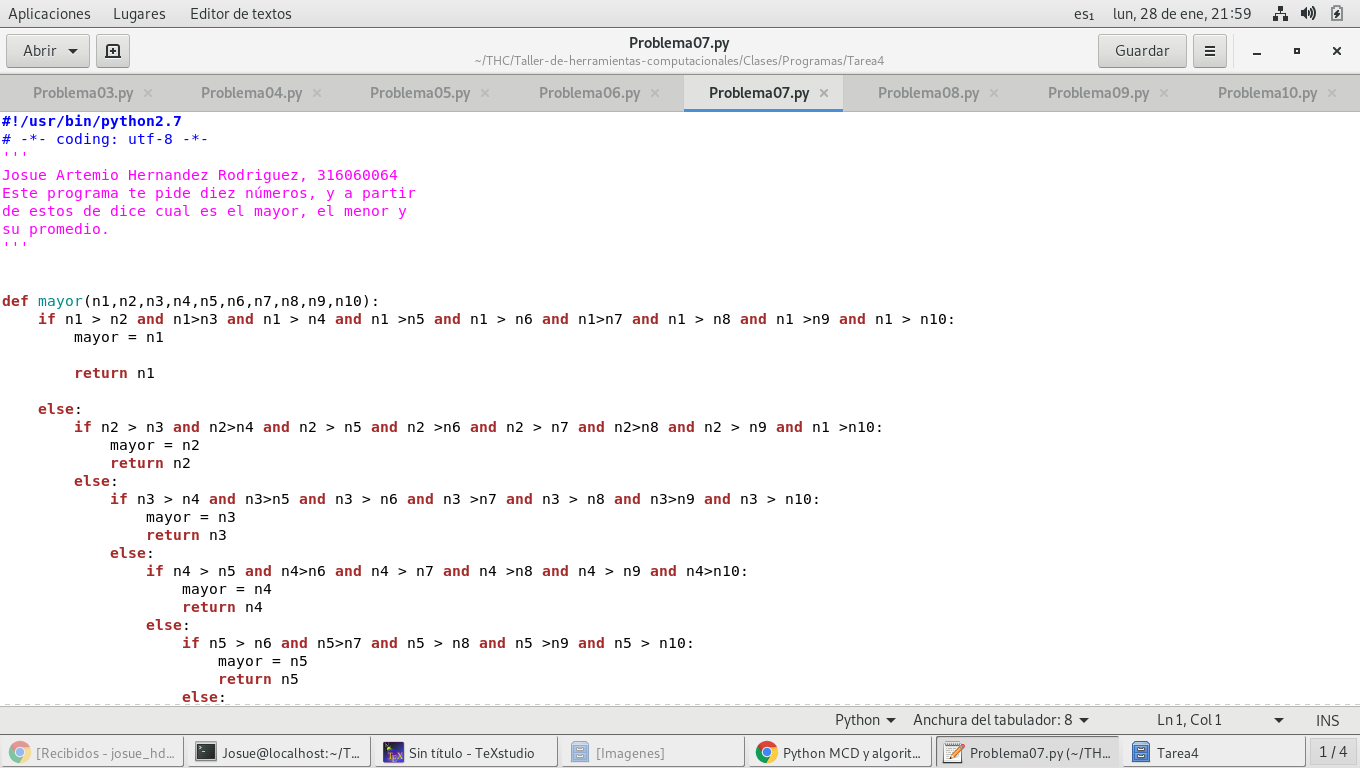
\includegraphics[scale=0.15]{pro07.png}
		
	\end{figure}
\begin{figure}[h]
	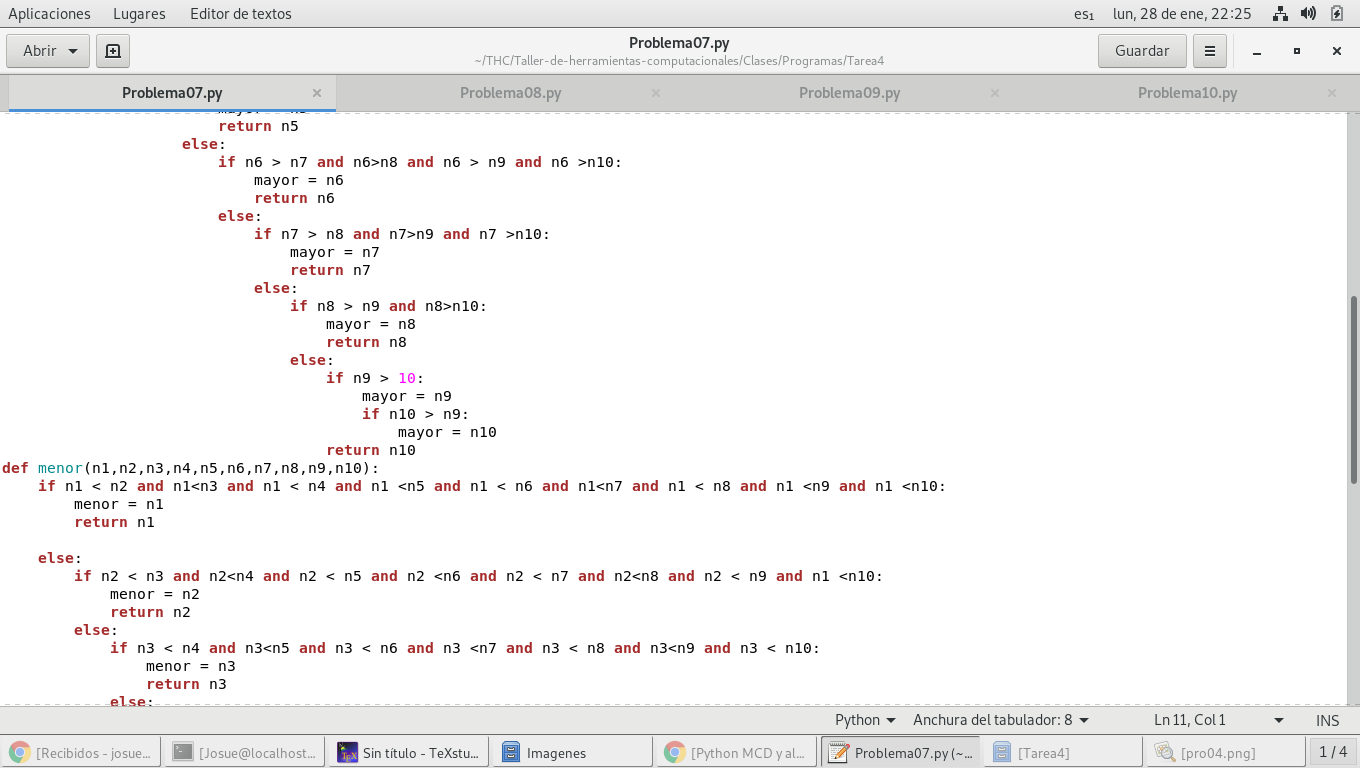
\includegraphics[scale=.15]{pro07_1.png}
	
\end{figure}
	\begin{figure}[h]
		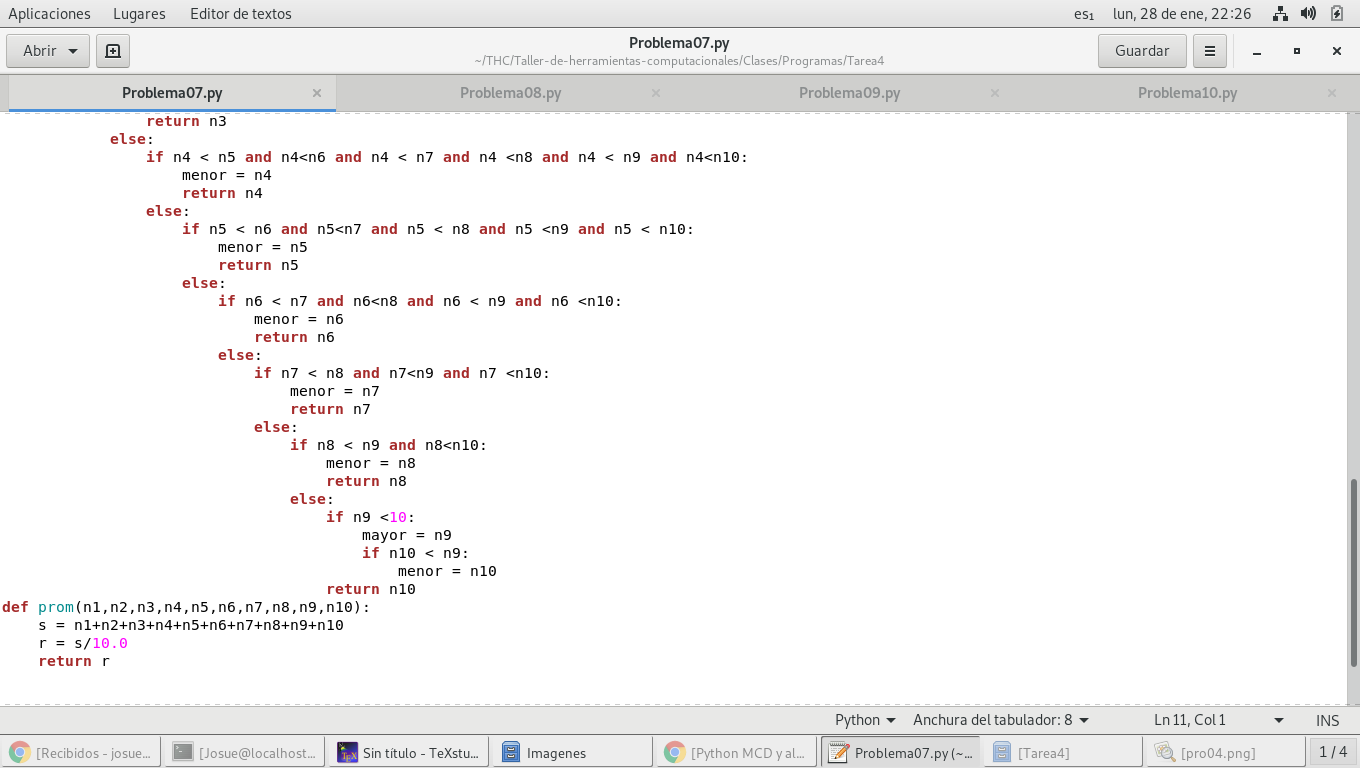
\includegraphics[scale=0.15]{pro07_2.png}
	\end{figure}
	
	
	
	
	
	
	
	
	
	
\end{document}
